% File: dedekind_cut_figure.tex
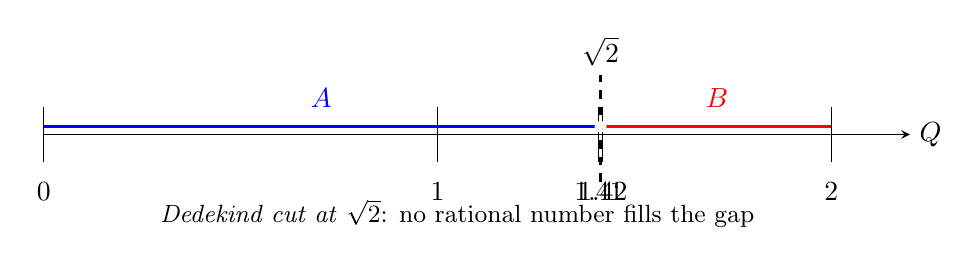
\begin{tikzpicture}[scale=5, >=stealth]
    \draw[->] (0,0) -- (2.2,0) node[right] {\(\mathbb{Q}\)};
    \foreach \x/\label in {0/0, 1/1, 1.41/1.41, 1.42/1.42, 2/2} {
      \draw[shift={(\x,0)}] (0pt,2pt) -- (0pt,-2pt) node[below=4pt] {\(\label\)};
    }
    \draw[very thick, blue] (0,0.02) -- (1.41,0.02) node[midway, above=3pt, blue] {\(A\)};
    \draw[very thick, red] (1.42,0.02) -- (2,0.02) node[midway, above=3pt, red] {\(B\)};
    \draw[dashed, thick] (1.4142, -0.12) -- (1.4142, 0.15);
    \node[above] at (1.4142, 0.15) {\(\sqrt{2}\)};
    \filldraw[white] (1.4142,0.02) circle (0.4pt);
    \node at (1.05, -0.2) {\small \textit{Dedekind cut at} \(\sqrt{2}\): no rational number fills the gap};
\end{tikzpicture}